
\begin{figure}[H]
	\centering
	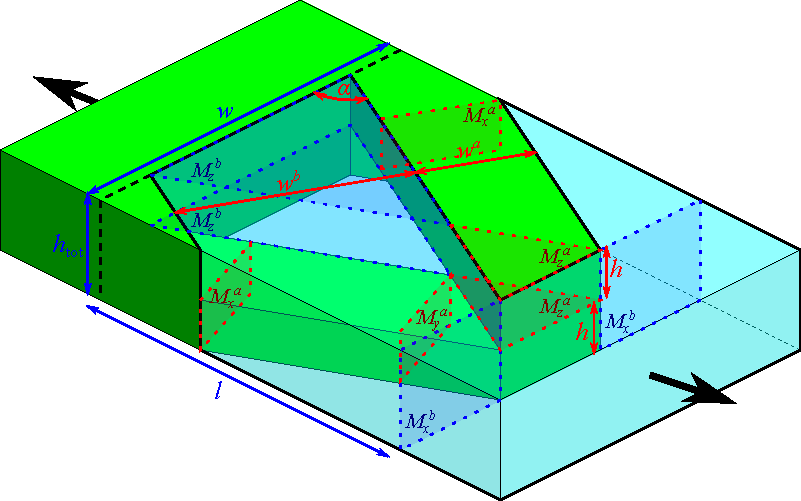
\includegraphics[width=\columnwidth]{sources/method/diagonal_model_v3.pdf}
	\caption{
		One diagonal unit cell connecting material $a$ (left) to material $b$ (right).
		Failure can happen along both the fingers ($M_x$), twice along one finger ($M_y$) or at the interface between the two fingers ($M_z$) for either material.}
	\label{fig:diagonal_model}
\end{figure}



\section{Diagonal design}

Another option is to place the fingers under an angle as shown in \autoref{fig:diagonal_model}.
There are four design variables: the finger width of both materials: $w^a$ and $w^b$, the finger rotation angle $\alpha$, and the layer thickness $h$.




The goal is to maximize the strength, while accounting for the failure modes in the constraints.
With that, the optimization problem can be formulated as follows:

\begin{align}
	& \max \frac{F \sin \alpha}{\left( w^a + w^b \right) 2h } \\
	\text{subject to:} & \nonumber \\
	w^m &\ge w_\text{min}^m \\
	h &\ge h_\text{min} \\
	\alpha_{min} &\le \alpha \le \alpha_{max}\\
	w^a + w^b &\le w_\text{max} \\
	\frac{ F \sin \alpha}{ w^m h } &\le \sigma^m_\text{yield} &&\text{ Tension failure } M_x^m \\
	\frac{ 3 F \cos \alpha }{ 4 w^m h_\text{c}} &\le \tau^m 			&&\text{ Shear failure } M_x^m \\
	\frac{ 3 F \sin \alpha \cos \alpha }{ \left(w^m \right)^2 } &\le \tau^m_\text{Z} 			&&\text{ Shear failure } M_z^m \\
	\frac{ 3 F w^b }{ 8 \sin \alpha \left(w^a \right)^2 h} & \le \sigma^a_\text{yield}			&&\text{ Bending failure } M_x^a \\
	\frac{ 3 F w^a }{ 8 \sin \alpha \left(w^b \right)^2 h} & \le \sigma^b_\text{yield}			&&\text{ Bending failure } M_x^b \\
	& \text{for both materials } && m \in \{a, b\} \nonumber
\end{align}

